
\documentclass{beamer}
\setbeamertemplate{itemize items}[circle]

\begin{document}

\begin{frame}
  \frametitle{Topological Data Analysis (TDA) Pipeline}

  \begin{itemize}
    \setlength\itemsep{1em}
    \item \textbf{Data Representation:} Represent the dataset as a point cloud in a high-dimensional space with a distance metric.
    \item \textbf{Simplicial Complex Construction:}
      \begin{itemize}
        \setlength\itemsep{0.5em}
        \item Connect points to form simplices.
        \item Aggregate simplices into a complex.
      \end{itemize}
    \item \textbf{Filtration:} Introduce a filtration parameter "t" and vary it.
    \item \textbf{Persistence:}
      \begin{itemize}
        \setlength\itemsep{0.5em}
        \item Track topological changes during filtration.
        \item Capture birth and death of topological features.
      \end{itemize}
  \end{itemize}
\end{frame}

\begin{frame}
  \frametitle{Topological Data Analysis (TDA) Pipeline (cont.)}

  \begin{itemize}
    \setlength\itemsep{1em}
    \item \textbf{Topological Summarization:} Summarize features using barcodes or persistence diagrams.
    \item \textbf{Interpretation and Visualization:}
      \begin{itemize}
        \setlength\itemsep{0.5em}
        \item Interpret results in the context of the original data.
        \item Visualize persistent homology using landscapes, heatmaps, etc.
      \end{itemize}
    \item \textbf{Validation and Application:}
      \begin{itemize}
        \setlength\itemsep{0.5em}
        \item Validate results against domain knowledge.
        \item Apply findings for insights into dataset structure.
      \end{itemize}
    \item \textbf{Integration:}
      \begin{itemize}
        \setlength\itemsep{0.5em}
        \item Cluster data based on topological features.
        \item Incorporate topological loss functions into machine learning. 
      \end{itemize}
  \end{itemize}
\end{frame}

\begin{frame}
\begin{columns}[t]
\column{.5\textwidth}
\centering
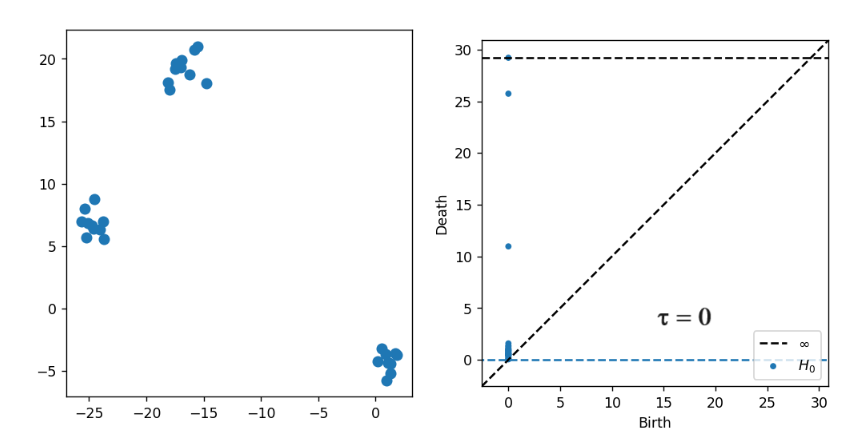
\includegraphics[width=5cm,height=3.5cm]{~/Personal-Writings/VR_Complex_T0.png}\\
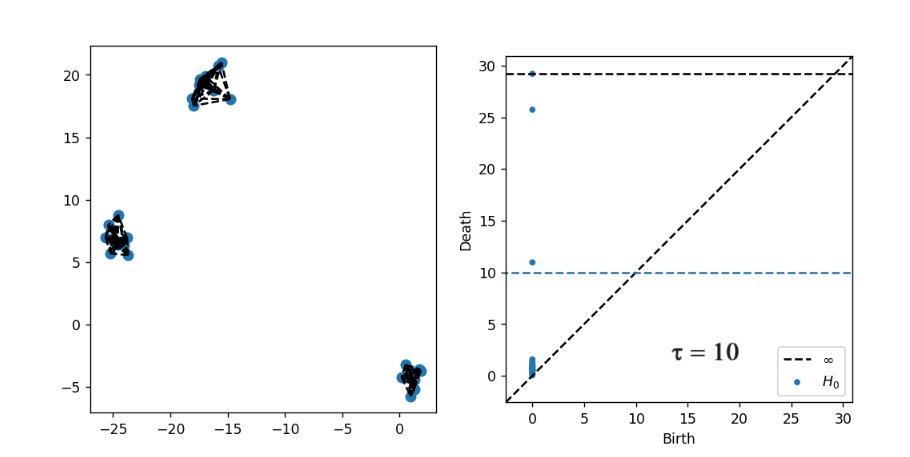
\includegraphics[width=5cm,height=3.5cm]{~/Personal-Writings/VR_Complex_T10.png}
\column{.5\textwidth}
\centering
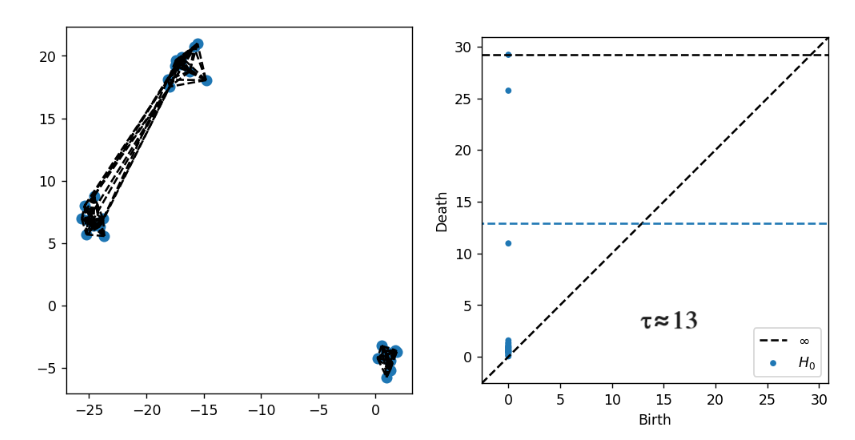
\includegraphics[width=5cm,height=3.5cm]{~/Personal-Writings/VR_Complex_T103.png}\\
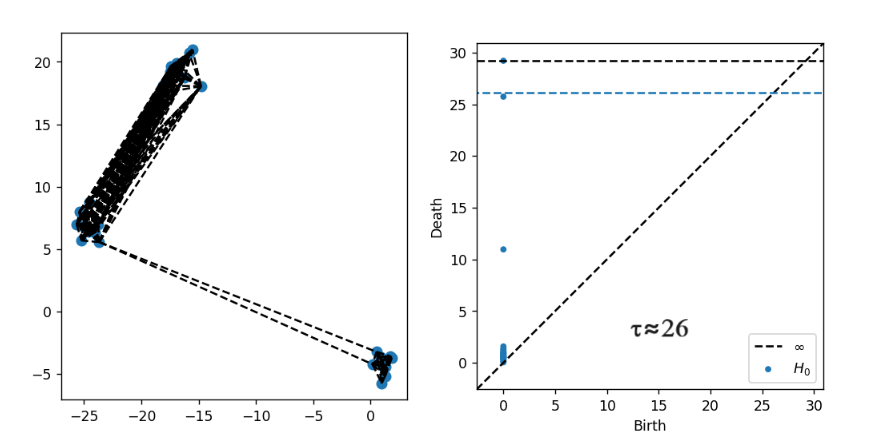
\includegraphics[width=5cm,height=3.5cm]{~/Personal-Writings/VR_Complex_T25.png}
\end{columns}
\end{frame}

\begin{frame}
  \begin{figure}
    \centering
    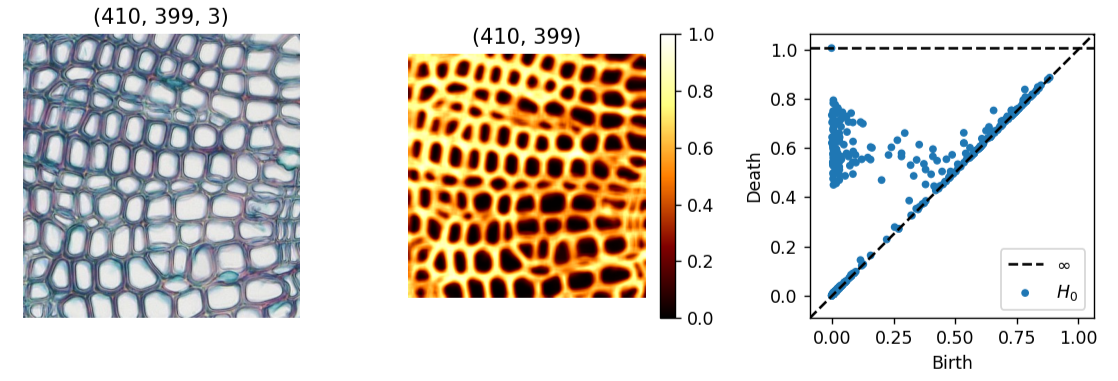
\includegraphics[width=10cm,height=5cm]{~/Personal-Writings/WoodCellHom.png }
    \caption{Homology of a wood cell wall. Filtered by pixel intensity.}
  \end{figure}
\end{frame}

\begin{frame}
  \begin{figure}
    \centering
    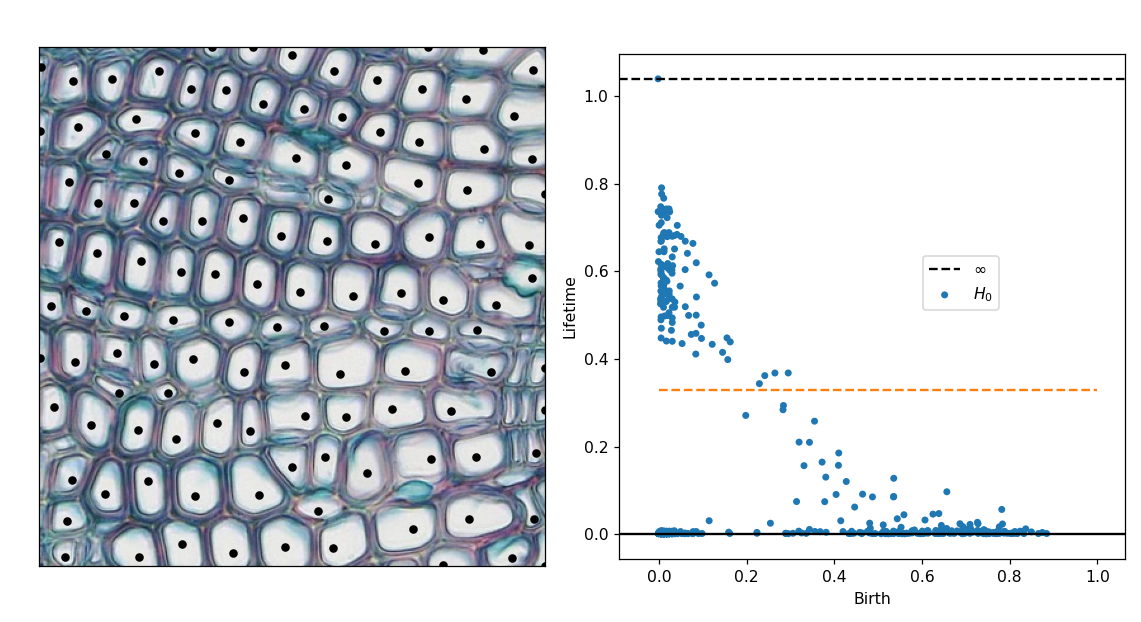
\includegraphics[width=10cm,height=5cm]{~/Personal-Writings/WoodCellFilter.png}
    \caption{Filtered wood cell wall.}
  \end{figure}
\end{frame}

\begin{frame}
  \begin{figure}
    \centering
    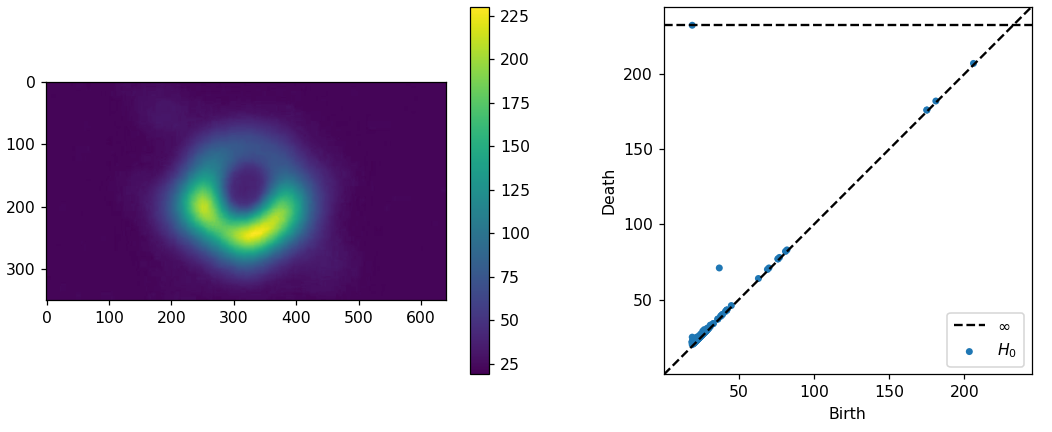
\includegraphics[width=10cm,height=5cm]{~/Personal-Writings/BlackHoleHole.png}
    \caption{An image of the black hole at the center of the galaxy M87.}
  \end{figure}
\end{frame}

\begin{frame}
  \begin{figure}
    \centering
    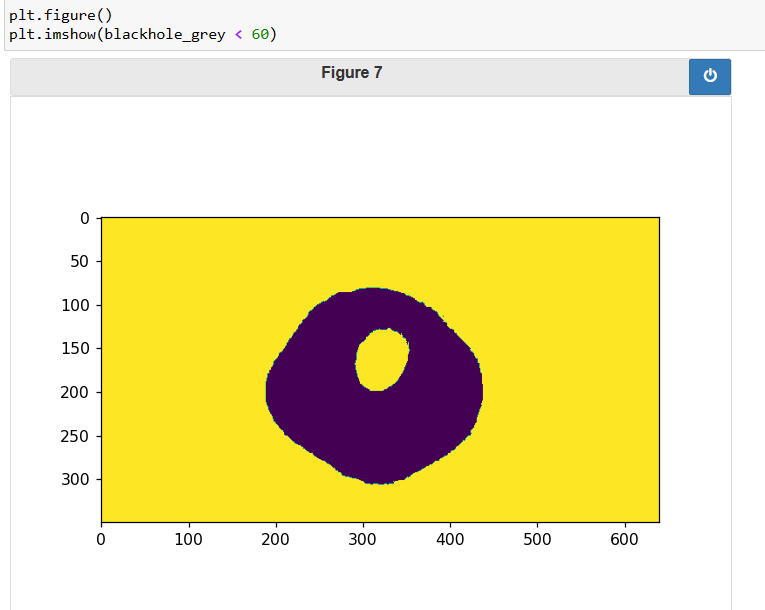
\includegraphics[width=10cm,height=5cm]{~/Personal-Writings/BlackHoleFilter.png}
    \caption{Proof that black holes do have holes}
  \end{figure}
\end{frame}

\begin{frame}
  \frametitle{TDA for Wave Data Pipeline}

  \begin{itemize}
    \setlength\itemsep{1em} % Adjust the separation between items
    \item \textbf{Data Representation:} Represent wave data as point clouds in a high-dimensional space.
    \item \textbf{Simplicial Complex Construction:}
      \begin{itemize}
        \setlength\itemsep{0.5em} % Adjust the separation between sub-items
        \item Need to know first what the data represents.
        \item Construct a simplicial filtration that captures the structure of the data.
      \end{itemize}
    \item \textbf{Lower Star Filtration:} Apply a lower star filtration method. Good for reconstruction of physical space.
    \item \textbf{Persistence:}
      \begin{itemize}
        \setlength\itemsep{0.5em} % Adjust the separation between sub-items
        \item Track changes during the filtration.
        \item Capture birth and death of topological features using persistent homology.
      \end{itemize}
  \end{itemize}
\end{frame}

\begin{frame}
  \frametitle{TDA for Wave Data Pipeline (cont.)}

  \begin{itemize}
    \setlength\itemsep{1em} % Adjust the separation between items
    \item \textbf{Topological Summarization:} Summarize persistent features using persistence landscapes.
    \item \textbf{Interpretation and Visualization:}
      \begin{itemize}
        \setlength\itemsep{0.5em} % Adjust the separation between sub-items
        \item Interpret results in the context of wave data.
        \item Visualize persistent homology using barcodes, persistence diagrams, etc.
      \end{itemize}
    \item \textbf{Validation and Application:}
      \begin{itemize}
        \setlength\itemsep{0.5em} % Adjust the separation between sub-items
        \item In some cases, "Persistent" topological features should correspond to wave features of high amplitude.
        \item The physical reality (obstructions) of the data should be reflected in the topological features of our data.
      \end{itemize}
    \item \textbf{Integration:}
      \begin{itemize}
        \setlength\itemsep{0.5em} % Adjust the separation between sub-items
        \item Incorporate in ML pipeline for obstruction / feature detection in noisy data.
        \item Object detection in sonar, radar, etc.
      \end{itemize}
  \end{itemize}
\end{frame}

\begin{frame}

  %% I want a conclusion slide that summarizes the main points of the talk.
  %% I want to end with a slide that shows the pipeline for TDA and how it can be applied to wave data.

  \frametitle{Conclusion}

Thank you for your time!
  \end{frame}


\end{document}

